\documentclass{article}
\usepackage[margin=0.9in]{geometry}
\usepackage{graphicx}
\usepackage{booktabs}
\usepackage{amsmath}
\usepackage{hyperref}
\usepackage{xcolor}
\usepackage{caption}
\usepackage{parskip}
\usepackage{enumitem}
\usepackage{array}
\usepackage{longtable}
\usepackage{tabularx}
\usepackage{float}
\usepackage{placeins}
\usepackage{listings}
\lstset{basicstyle=\ttfamily\footnotesize, breaklines=true, columns=fullflexible, frame=single, framerule=0.2pt}
\setlist{nosep, leftmargin=1.5em}
\hypersetup{colorlinks=true, linkcolor=blue, urlcolor=blue, citecolor=blue}
\captionsetup{font=small, labelfont=bf}
\renewcommand{\topfraction}{0.9}
\renewcommand{\bottomfraction}{0.8}
\renewcommand{\textfraction}{0.07}
\renewcommand{\floatpagefraction}{0.85}
\setcounter{topnumber}{3}
\setcounter{totalnumber}{5}
\newcommand{\us}{\,$\mu$s}

\title{Project 3: SSD Performance Profiling\\[3pt]\large ECSE 4320/6320 Advanced Computer Systems}
\author{Demetrios Sotirelis}
\date{\today}

\emergencystretch=3em
\begin{document}
\maketitle

\begin{abstract}
This report profiles a 1\,TB Crucial MX500 solid-state drive (SSD) on a Serial Advanced Technology Attachment (SATA) interface, using direct input/output (I/O) on a scratch file in a dedicated 1.6\,GiB partition. The Flexible I/O tester (FIO) 3.43 and an independent C++ tool ran 12 stages, more than 500 runs and 2.1\,TB of writes. At queue depth (QD) 1, a 4\,KiB random read takes 92\us\ and a write 36\us, because the drive acknowledges writes from its cache. Throughput in I/O operations per second (IOPS) rises with queue depth until the drive's 32-entry Native Command Queuing (NCQ) queue is full; beyond that only latency grows, and large transfers hit the SATA link limit of about 560\,MB/s. A 70/30 read/write mix collapses to 38\% of read-only throughput. Long runs reveal what short ones hide. Sequential writes hold 505\,MB/s for 900\,s, but sustained random writes fall off a cliff after 99--316\,GB, most likely from garbage collection, and sustained 4\,KiB reads of a small range step down by up to a third after about 14--17 million reads. Buffered I/O, a sparse file or a synchronous engine inflate results 3 to 70 times. A summary of results, a map from the grading rubric to this report and a requirements checklist are in the appendices.
\end{abstract}

\section{Reproducibility and data hygiene}\label{sec:repro}
The repository holds the FIO job file and raw output of every run (\texttt{data/raw/jobs|json|logs|ref}), the parsed data (\texttt{data/processed}), the scripts (\texttt{scripts/}) and the C++ tool (\texttt{src/}). Run from an elevated PowerShell, because the Self-Monitoring, Analysis and Reporting Technology (SMART) counters need administrator rights, on a machine with a dedicated test partition as described in Sec.~\ref{sec:safety}; \texttt{run\_fio.py} refuses to start otherwise.
\begin{lstlisting}
powershell -File scripts\run_all.ps1     # build, record environment, FIO stages 1-12, C++ reference runs, sanity checks, plots (about 5 h)
python scripts\run_fio.py --stages 4,5   # any subset of stages; resume-safe (finished JSON files are skipped)
python scripts\process_and_plot.py       # raw JSON -> data\processed, results\fig*.png, report\generated\*.tex
cd report; pdflatex report.tex           # twice, so that cross-references resolve
\end{lstlisting}
In run order, the stages are the queue-depth-1 baselines (stage 1), the block-size matrix (2), the read/write mix (3), the queue-depth and \texttt{numjobs} sweep (4), tail latency (5), address range (6), data pattern (7), misleading setups (8), sustained writes (9), read stability (10), read-step triggers (12) and the write cliff (11). The fresh-state stages run first and the write cliff last, because heavy writes change the device state. FIO is extracted from the official installer to \texttt{\%LOCALAPPDATA\%\char92Programs\char92fio-extracted} instead of being installed, because installing needs administrator rights.

All raw FIO output, per-second logs, job start and end times, the SMART log, operating-system counter logs and the C++ tool's output are kept, and the scripts are resume-safe. While the campaign ran, hardware-counter pipelines for Projects~1 and~2 were validated on the same machine; the 57 jobs of stage 2 whose run time overlapped that work were deleted and re-run afterwards (\texttt{perturbed\_jobs\_rerun.txt}).

Across the three trials of a configuration, the median coefficient of variation of IOPS is 0.1--1.0\% per stage. The largest values are state effects, not noise, namely sustained reads that change plateau (Sec.~\ref{sec:readstab}) and the 21 of 555 run-directions with a stall, meaning a maximum latency above 100\,ms and above 50 times the median, listed in \nolinkurl{data/processed/stall_census.csv}. Runs with a stall are listed rather than excluded. A median over three trials resists a single stalled trial but not three, so the queue-depth-1 reference for sequential writes comes from the 5-trial baseline.

\section{Methodology}\label{sec:method}
\subsection{Safe setup}\label{sec:safety}
The benchmark runs on a dedicated New Technology File System (NTFS) partition, \texttt{T:}, labelled ``Testing'', which is 1.62\,GiB at the end of the physical SSD that also holds the data volume \texttt{G:}, at a 1\,MiB-aligned offset. Only one 1500\,MiB scratch file, \texttt{T:\char92ssdbench\char92fio.dat}, is created and rewritten, with file-level direct I/O, which requires sector-aligned offsets and sizes \cite{msfilebuf}. There are no raw disk or volume handles, no formatting or partitioning, and \texttt{G:} is never opened.

The benchmark code includes checks that ensure it is only running on a path \texttt{T:\char92} with appropriate file size limits.

All block sizes are multiples of 4\,KiB and random offsets are block-aligned \cite{fiodoc}. The whole file is written twice sequentially with incompressible data before the first read test, because NTFS returns zeros for never-written ranges without touching the SSD (Sec.~\ref{sec:pitfalls}).

\subsection{Environment}\label{sec:env}
{\small
\begin{longtable}{p{2.6cm}p{13.4cm}}
\toprule
Device & Crucial \texttt{CT1000MX500SSD1}, 1\,TB SSD on SATA III at 6\,Gb/s, firmware M3CR043, 21\,512 power-on hours. Triple-level-cell (TLC) flash with a dynamic random-access memory (DRAM) cache and a dynamic single-level-cell (SLC) write cache whose size follows the free capacity \cite{computerbase}; NCQ depth 32 \cite{ncq}; 512\,B sectors. The manufacturer gives 560/510\,MB/s sequential and 360 terabytes written (TBW) of endurance \cite{ocinside}; up to 95\,k/90\,k random 4\,KiB IOPS from a retailer listing \cite{geektopia}. \\
File system & NTFS file on the dedicated 1659\,MiB partition \texttt{T:}, 4096\,B clusters, compression off. Direct I/O; the device write cache is enabled and not power-protected. A 1500\,MiB file, with a 1024\,MiB test range unless stated. \\
I/O generator & FIO 3.43 with the \texttt{windowsaio} engine, which uses I/O completion ports; block-aligned random offsets, every I/O refilled with incompressible random data, a fixed seed per trial. An independent C++/Win32 tool for the cross-check at queue depth 1 and for the pitfalls, built with g++ 16.2.0 from MSYS2; Python 3.12 for parsing and plots. All versions are recorded in \texttt{results/environment.txt}. \\
Host & AMD Ryzen~9 9950X with simultaneous multithreading (SMT), 31\,GiB of random-access memory (RAM), Windows~11 build 26200, High performance power plan, recorded but not changed. FIO threads are not pinned; host effects are checked with operating-system counters (Sec.~\ref{sec:readstab}). Background applications were running, so their per-I/O cost is part of every number.\\
Temperature & SMART counters \cite{msstorrel} read after every job and every 30\,s during runs of at least 120\,s. No polling during short jobs, because a SMART query is a non-queued command, and polling every 2\,s stalled the drive for about 0.5\,s on one poll in three. During sustained writes at queue depth 32 the queries mostly fail, because the command cannot pass a full queue. \\
Repetitions & 3 trials per configuration, 5 for the queue-depth-1 baselines, 2 for the 45\,s tail runs and 1 for the sustained runs, in trial-major order so that slow drift cannot bias one configuration; 6--20\,s per point after a 2\,s ramp; tables show medians, plots the min--max of the trials. \\
\bottomrule
\end{longtable}
}

\subsection{Correctness validation}\label{sec:valid}
The independent C++ tool, \texttt{ref\_qd1.cpp}, with its own timer and percentiles, reproduces FIO's median latency at queue depth 1 within 7\% for all four baselines (Tab.~\ref{tab:zq}). On all runs, $\text{MB/s}=\text{IOPS}\times\text{block size}$ holds within 1.1\% over 555 run-directions, and $N=\text{IOPS}\times\text{mean latency}$ equals the requested queue depth with a median ratio of 0.998 over 331 runs. A parser self-test on synthetic FIO output with known values caught a missing-percentile case. As physical sanity checks, the read plateau equals the SATA~III payload limit and the published sequential rate, the random-read peak is within 5\% of the published figure, and the buffered and sparse-file results have the magnitude of RAM, as they must. During the read-stability runs, the operating system's \texttt{PhysicalDisk} counters report reads per second equal to FIO's IOPS, zero writes and 30--32 requests outstanding. The effect of SMART polling on the benchmark was measured before the campaign and the poller redesigned.

\section{Hypotheses}\label{sec:hyp}
{\small
\begin{longtable}{@{}lp{7.7cm}p{7.7cm}@{}}
\toprule
& \textbf{Prediction} & \textbf{Outcome} \\
\midrule
\endhead
1 & At QD1, a SATA drive with TLC flash reads a random 4\,KiB page in 80--120\us; writes acknowledged from the controller's buffer take under 50\us; a 128\,KiB sequential read takes 300--400\us, including about 240\us\ of transfer. & Held for 4\,KiB requests; 128\,KiB sequential reads took 500--830\us, depending on how the range was last written (Sec.~\ref{sec:anomalies}). \\
2 & IOPS fall and MB/s rise with block size until the 6\,Gb/s link saturates near 550--560\,MB/s; sequential is at least as fast as random. & Held (Sec.~\ref{sec:bs}). \\
3 & IOPS grow roughly linearly with QD until the drive's internal parallelism or its 32-entry NCQ queue is exhausted; latency then grows linearly, as Little's Law requires, and the knee lies near $N^{*}=L_{1}X_{\max}$, the QD1 latency times the maximum IOPS. & Held for saturation at the NCQ depth, but the knee lies one to two doublings above $N^{*}$, not near it (Sec.~\ref{sec:knee}). \\
4 & Flash reads wait behind program operations, so any mix with writes does worse than the weighted average of the pure workloads. & Held (Sec.~\ref{sec:mix}). \\
5 & Flushes and garbage collection give writes a worse tail than reads, and tails inflate once the queue is saturated. & Held (Sec.~\ref{sec:tail}). \\
6 & Throughput does not depend on the logical block address (LBA) range from 1\,MiB to 1500\,MiB, far below the drive's cached mapping table and its SLC write cache. & Held for writes; reads lost a little throughput at the largest ranges (Sec.~\ref{sec:ws}). \\
7 & Sustained writes slow once the SLC cache is exhausted, but only if the unique valid data exceed the cache; overwriting the same 1500\,MiB keeps them far below, so no cliff. & Right for sequential writes, wrong for random writes, which show a cliff, most likely from garbage collection rather than SLC exhaustion (Sec.~\ref{sec:state}). \\
8 & Buffered I/O and unwritten files inflate IOPS by orders of magnitude, and synchronous engines ignore \texttt{iodepth}. & Held (Sec.~\ref{sec:pitfalls}). \\
9 & Any change in the 4\,KiB random-read ceiling under sustained load follows the drive's temperature. & Rejected, since the read steps do not follow temperature (Sec.~\ref{sec:readstab}). \\
\bottomrule
\end{longtable}
}

\section{Results}\label{sec:results}
\subsection{Latency at queue depth 1}\label{sec:zqsec}
\begin{table}[!htb]\centering\small\begin{tabular}{lrrrrrrrr}
\toprule
QD=1 workload & IOPS & MB/s & mean & p50 & p95 & p99 & p99.9 & C++ ref p50 / p99 \\
 & & & \multicolumn{4}{c}{FIO latency ($\mu$s)} & & ($\mu$s) \\
\midrule
4 KiB random read & 10,604 & 43.4 & 94 & 92 & 114 & 127 & 198 & 92 / 106 \\
4 KiB random write & 25,598 & 104.9 & 39 & 36 & 58 & 153 & 167 & 33 / 152 \\
128 KiB seq read & 1,340 & 175.7 & 746 & 733 & 889 & 979 & 1106 & 709 / 976 \\
128 KiB seq write & 3,283 & 430.3 & 302 & 285 & 371 & 395 & 485 & 274 / 396 \\
\bottomrule
\end{tabular}

\caption{Queue depth 1, direct I/O, 1\,GiB range, medians of 5 trials of 20\,s. Latency is the total latency reported by FIO; the last column is the independent C++ tool's median and 99th percentile.}\label{tab:zq}\end{table}
\begin{figure}[!htb]\centering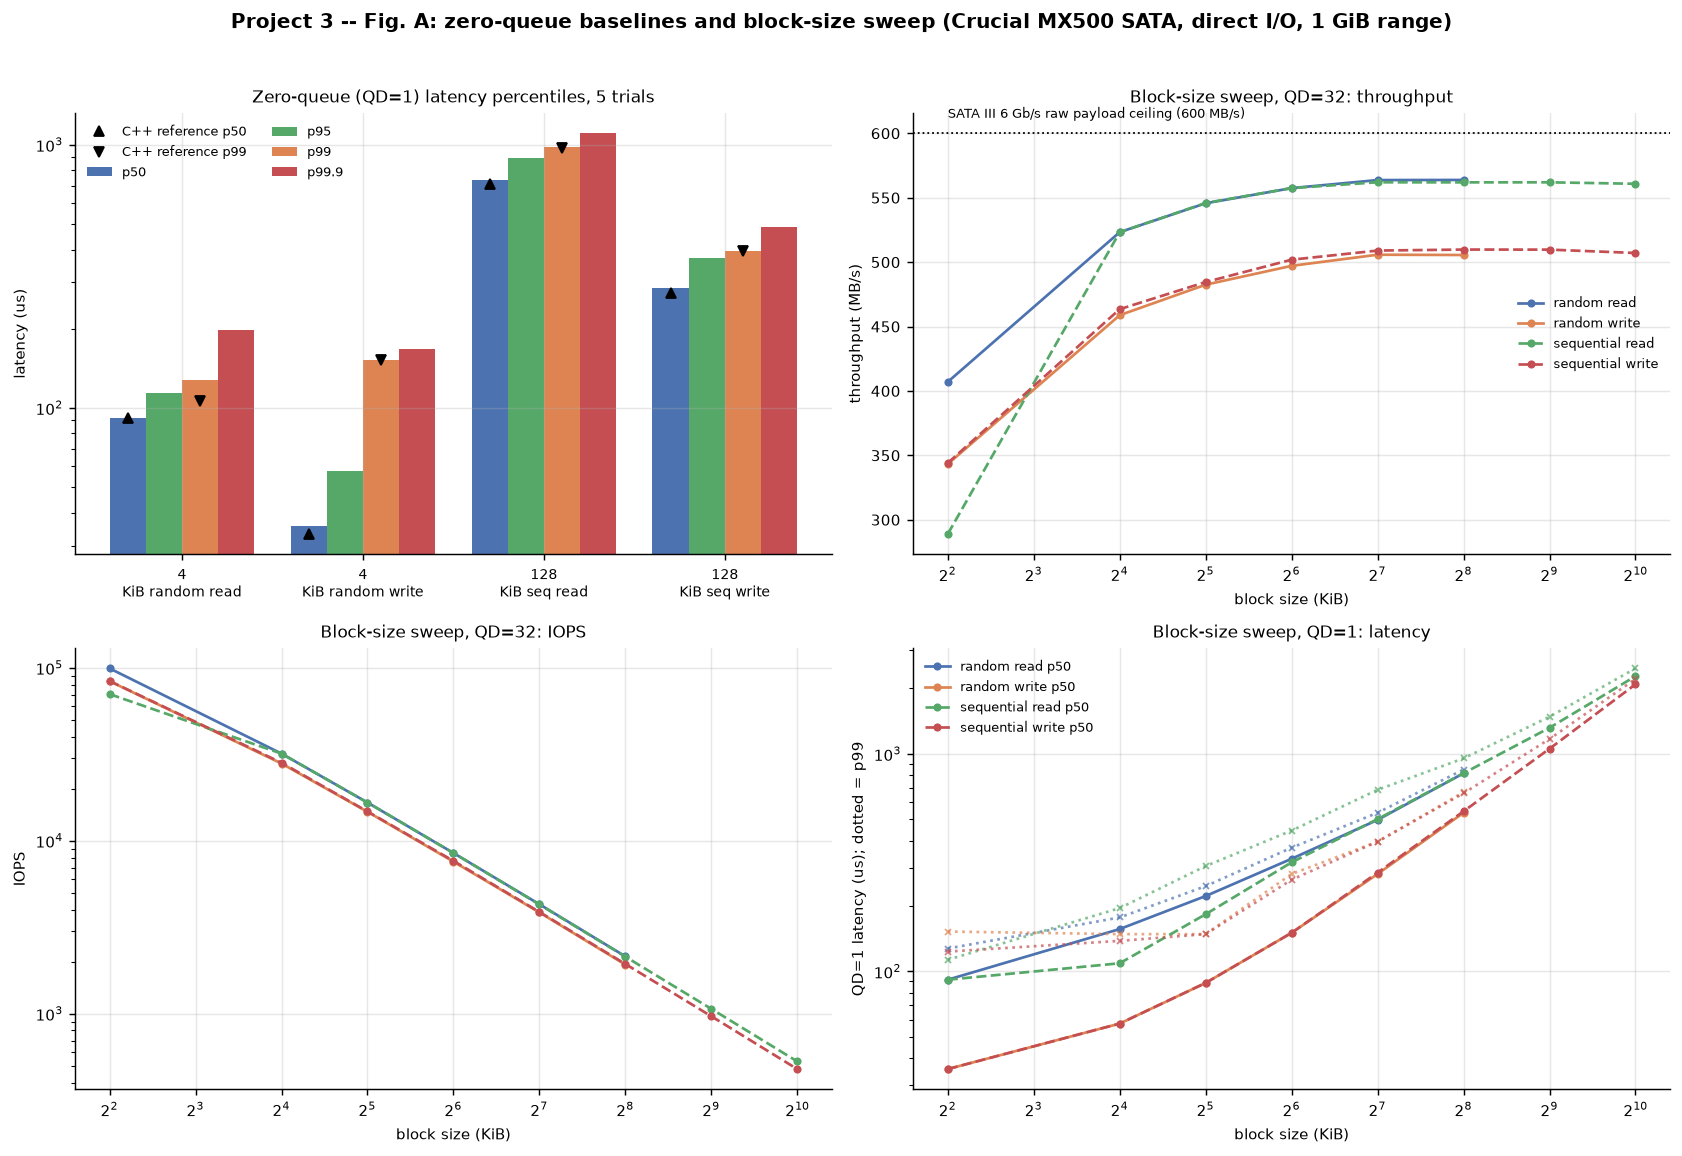
\includegraphics[width=\linewidth]{../results/figA_baselines_and_blocksize.png}
\caption{Latency percentiles at queue depth 1, FIO as bars and the C++ tool as triangles (top left); block-size sweep at queue depth 32 (top right, bottom left); block-size sweep at queue depth 1, medians solid and 99th percentiles dotted (bottom right). Direct I/O and a 1\,GiB range throughout.}\label{fig:A}\end{figure}
A random 4\,KiB read at QD1 has a tight latency distribution, which limits a synchronous reader to about 10.6\,k IOPS (Tab.~\ref{tab:zq}). A random write is faster, because the controller acknowledges it from its volatile write cache before programming flash \cite{msfilebuf}, but its tail is heavier, with at least 1\% of writes wait for something internal. A 128\,KiB sequential write takes little more than its transfer time over the link, while a read takes more than twice as long here, because the range was last written by 4\,KiB random writes (Sec.~\ref{sec:anomalies}). The C++ tool agrees within 7\% on every median and on three of the four 99th percentiles (p99); FIO reports a higher 4\,KiB read tail that the tool does not confirm. Tails also vary between runs. Over the campaign's 31 direct 4\,KiB QD1 read runs the 95th percentile (p95) is bimodal, and for writes the p95 and the 99.9th percentile (p99.9) jump between two levels, so Tab.~\ref{tab:zq}, from stage 1, differs from the tail table of Sec.~\ref{sec:tail}.

\FloatBarrier
\subsection{Block size and access pattern}\label{sec:bs}
\begin{table}[!htb]\centering\footnotesize\begin{tabular}{lrrrrrrr}
\toprule
 & & \multicolumn{3}{c}{QD=1} & \multicolumn{3}{c}{QD=32} \\
pattern & bs & IOPS & MB/s & p50 $\mu$s & IOPS & MB/s & mean $\mu$s \\
\midrule
random read & 4k & 10,627 & 44 & 92 & 99,367 & 407 & 320 \\
 & 16k & 6,441 & 106 & 157 & 31,932 & 523 & 1002 \\
 & 32k & 4,627 & 152 & 222 & 16,647 & 546 & 1922 \\
 & 64k & 3,049 & 200 & 330 & 8,501 & 557 & 3763 \\
 & 128k & 1,999 & 262 & 498 & 4,295 & 564 & 7444 \\
 & 256k & 1,232 & 323 & 815 & 2,145 & 564 & 14895 \\
\addlinespace
random write & 4k & 26,198 & 107 & 36 & 83,795 & 343 & 380 \\
 & 16k & 15,463 & 253 & 58 & 27,997 & 459 & 1142 \\
 & 32k & 10,249 & 336 & 89 & 14,718 & 482 & 2173 \\
 & 64k & 5,787 & 379 & 151 & 7,580 & 497 & 4218 \\
 & 128k & 3,319 & 435 & 281 & 3,853 & 506 & 8296 \\
 & 256k & 1,715 & 450 & 537 & 1,923 & 506 & 16608 \\
\addlinespace
sequential read & 4k & 10,869 & 45 & 92 & 70,538 & 289 & 452 \\
 & 16k & 7,991 & 131 & 109 & 31,930 & 523 & 1002 \\
 & 32k & 5,120 & 168 & 183 & 16,654 & 546 & 1921 \\
 & 64k & 3,094 & 203 & 317 & 8,501 & 557 & 3763 \\
 & 128k & 1,924 & 252 & 502 & 4,282 & 562 & 7467 \\
 & 256k & 1,218 & 319 & 815 & 2,138 & 562 & 14945 \\
 & 512k & 749 & 393 & 1319 & 1,067 & 562 & 29920 \\
 & 1m & 437 & 458 & 2277 & 530 & 561 & 60097 \\
\addlinespace
sequential write & 4k & 25,935 & 106 & 36 & 83,991 & 344 & 379 \\
 & 16k & 15,351 & 252 & 58 & 28,282 & 463 & 1131 \\
 & 32k & 10,079 & 330 & 89 & 14,781 & 485 & 2163 \\
 & 64k & 5,851 & 383 & 151 & 7,653 & 502 & 4178 \\
 & 128k & 3,283 & 430 & 285 & 3,878 & 509 & 8243 \\
 & 256k & 1,742 & 457 & 545 & 1,939 & 510 & 16471 \\
 & 512k & 906 & 475 & 1057 & 967 & 510 & 32984 \\
 & 1m & 463 & 486 & 2089 & 478 & 507 & 66461 \\
\addlinespace
\bottomrule
\end{tabular}

\caption{Block sizes from 4 to 256\,KiB for random and sequential access, plus 512\,KiB and 1\,MiB sequential, for reads and writes; medians of 3 trials. Throughput and latency come from the same runs, at queue depth 1 and 32.}\label{tab:bs}\end{table}
IOPS, MB/s and latency tell different stories (Tab.~\ref{tab:bs}, Fig.~\ref{fig:A}). At QD32, small requests are limited by per-command overhead and deliver many IOPS but little bandwidth, while requests of 64\,KiB and up are limited by the SATA link. Past that point larger blocks only add latency, as mean latency grows in proportion to block size, because 32 requests share the same link. Writes saturate slightly lower than reads. At QD1 a request costs a fixed command time plus its size divided by the transfer rate, so MB/s grows with block size; even 1\,MiB requests cannot keep the link busy with only one outstanding.

Random and sequential writes are identical at every size and QD, since a flash drive has no seek. Reads agree at QD32 from 16\,KiB up and at QD1 from 64\,KiB up. Below that, sequential QD1 reads are faster, consistent with the controller prefetching the next flash pages of a sequential stream, which was not tested; 4\,KiB sequential reads at QD32 are much slower than random ones (Sec.~\ref{sec:anomalies}).

\FloatBarrier
\subsection{Read/write mix}\label{sec:mix}
\begin{table}[H]\centering\small\begin{tabular}{lrrrrrrr}
\toprule
mix (4 KiB random) & QD & IOPS & MB/s & read p50 / p99 $\mu$s & write p50 / p99 $\mu$s \\
\midrule
100R & 1 & 10,509 & 43 & 92 / 125 & -- \\
100R & 32 & 98,887 & 405 & 313 / 514 & -- \\
100W & 1 & 25,324 & 104 & -- & 36 / 153 \\
100W & 32 & 84,994 & 348 & -- & 371 / 403 \\
70R30W & 1 & 12,645 & 52 & 91 / 127 & 36 / 77 \\
70R30W & 32 & 37,670 & 154 & 782 / 1958 & 700 / 1843 \\
50R50W & 1 & 14,501 & 59 & 91 / 136 & 36 / 77 \\
50R50W & 32 & 40,147 & 164 & 774 / 1958 & 692 / 1860 \\
\bottomrule
\end{tabular}

\caption{4\,KiB random I/O over a 1\,GiB range. IOPS and MB/s are read-plus-write totals, latencies are per direction as median and 99th percentile; medians of 3 trials.}\label{tab:mix}\end{table}
At QD32 the 70/30 read/write mix delivers only 38\% of the read-only IOPS, and the read p99 nearly quadruples (Tab.~\ref{tab:mix}). A flash die that is programming cannot serve reads, so reads and writes block one another, and write-buffer flushes compete with reads. At QD1 the interference is mild, so the damage is a queueing effect among concurrent requests, not a per-request penalty. The 128\,KiB sequential mixes at QD4 behave the same way, falling from the link limit to about 400\,MB/s.

\FloatBarrier
\subsection{Queue depth, knee and Little's Law}\label{sec:knee}
\begin{figure}[!htb]\centering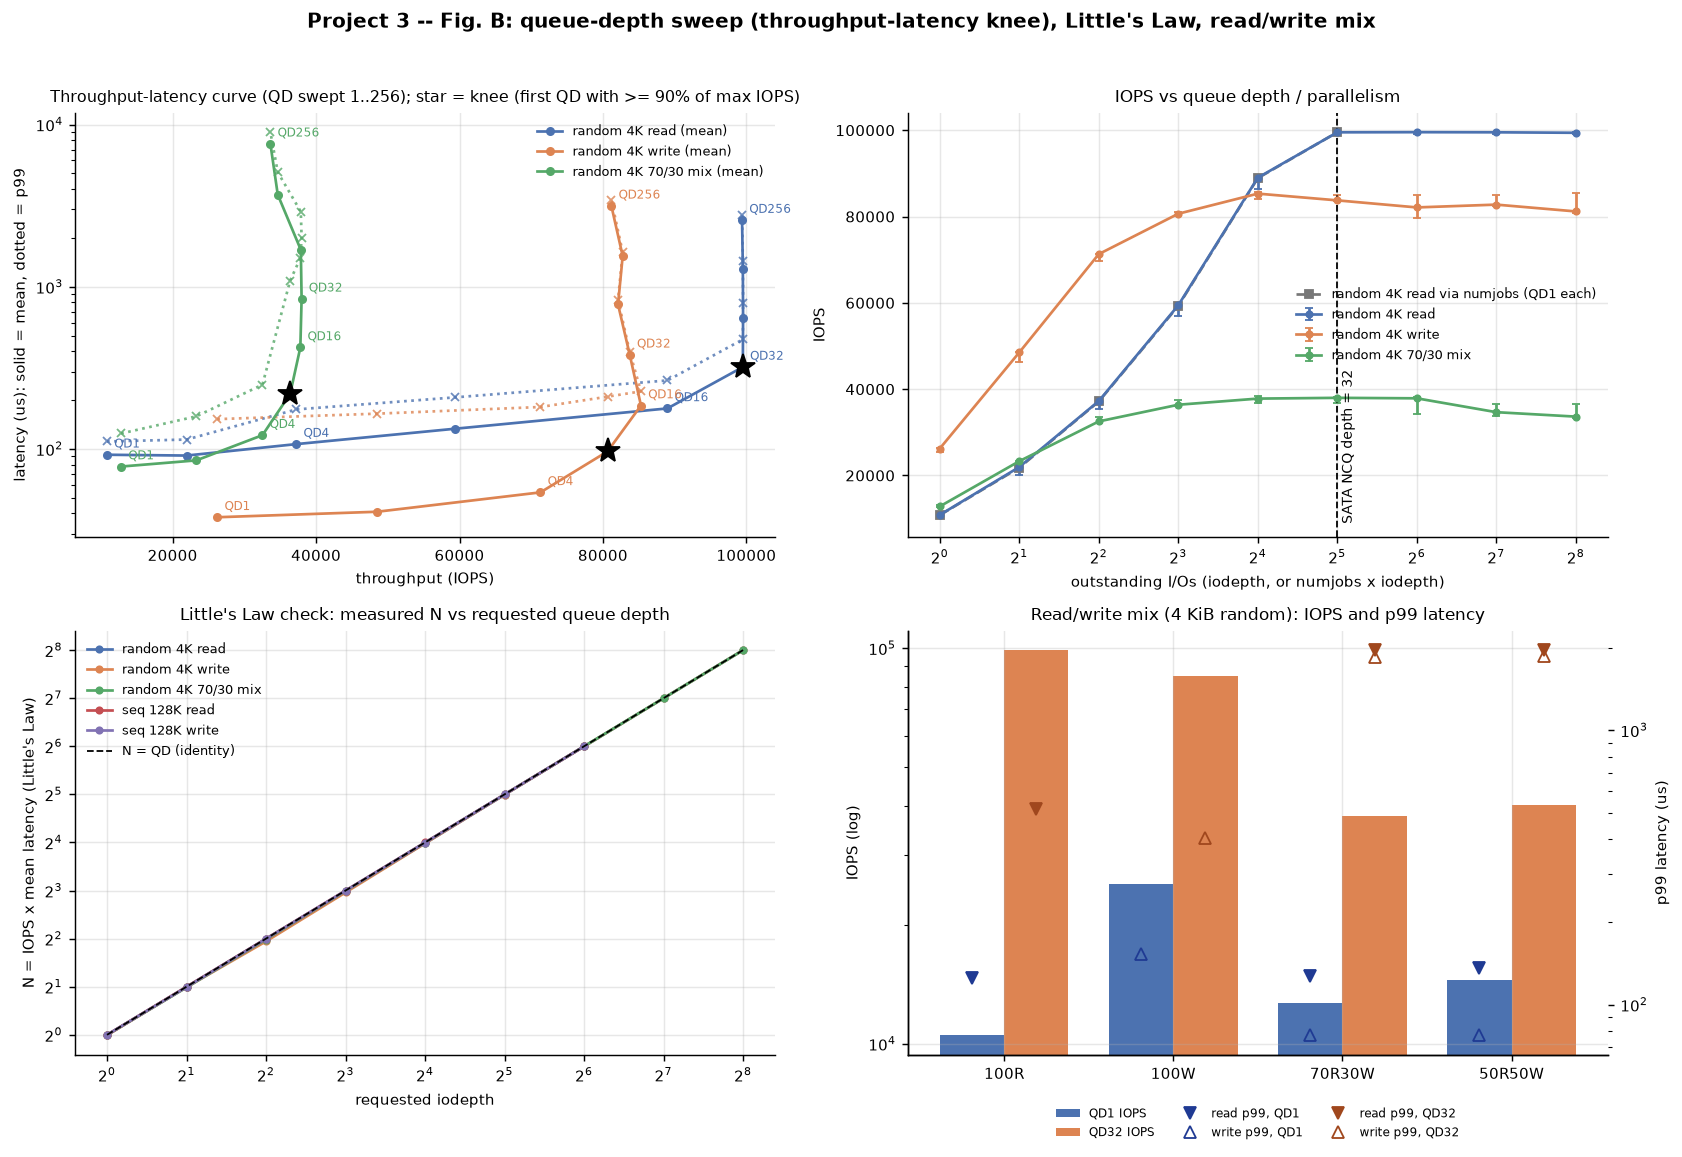
\includegraphics[width=\linewidth]{../results/figB_qd_sweep_and_mix.png}
\caption{Throughput against latency, mean solid and 99th percentile dotted, for queue depths 1--256, with stars at the knee, the first queue depth with at least 90\% of the maximum (top left); IOPS against outstanding I/Os, with min--max error bars over 3 trials, grey points for the same read workload built with \texttt{numjobs} instead of \texttt{iodepth}, and a dashed line at the depth of NCQ (top right); $N=\text{IOPS}\times\text{mean latency}$ against the requested depth (bottom left); IOPS and 99th percentile by mix (bottom right).}\label{fig:B}\end{figure}
\begin{table}[!htb]\centering\small\resizebox{\linewidth}{!}{\begin{tabular}{lrrrrrrrr}
\toprule
workload & QD1 IOPS & max IOPS & MB/s at max & $N^{*}=L_1 X_{\max}$ & QD for 90\% & mean latency there & QD for 98\% & latency $\times$ at top QD \\
\midrule
random 4K read & 10,604 & 99,543 & 408 & 9.4 & 32 & 320 $\mu$s & 32 & 27$\times$ (QD 256) \\
random 4K write & 25,598 & 85,304 & 349 & 3.3 & 8 & 96 $\mu$s & 16 & 81$\times$ (QD 256) \\
random 4K 70/30 mix & 12,816 & 37,982 & 156 & 3.0 & 8 & 218 $\mu$s & 16 & 98$\times$ (QD 256) \\
seq 128K read & 1,340 & 2,951 & 387 & 2.2 & 4 & 1355 $\mu$s & 4 & 29$\times$ (QD 64) \\
seq 128K write & 3,283 & 3,856 & 507 & 1.2 & 2 & 538 $\mu$s & 4 & 55$\times$ (QD 64) \\
\bottomrule
\end{tabular}
}
\caption{Knee analysis. $N^{*}=L_{1}X_{\max}$, with $L_{1}$ the mean latency at queue depth 1 and $X_{\max}$ the maximum IOPS, is the number of requests the drive must overlap to deliver $X_{\max}$. The 90\% and 98\% columns give the first queue depth that reaches that fraction of the maximum.}\label{tab:knee}\end{table}
Random-read IOPS grow almost linearly up to QD8 and plateau at QD32, the NCQ depth (Fig.~\ref{fig:B}, Tab.~\ref{tab:knee}); beyond that each doubling of QD doubles the mean latency for no gain. A sweep built with \texttt{numjobs} instead of \texttt{iodepth} lies on the same curve, so queue depth means outstanding requests however they are generated. Random writes saturate sooner, at QD8, because the controller acknowledges them early. The 70/30 mix saturates at QD8 with by far the worst tail. Sequential 128\,KiB I/O saturates at QD2--4; its read plateau here, about 390\,MB/s, is below the link limit because this stage read a range last written by 4\,KiB random writes (Sec.~\ref{sec:anomalies}).

By Little's Law \cite{little1961} with measured mean latency, $N=\text{IOPS}\times\text{latency}$ has a median ratio of 0.998 to the requested depth over 331 runs, which only confirms that FIO keeps that many requests in flight. The informative use is predictive, since $N^{*}=L_{1}X_{\max}$ is the drive's internal parallelism as seen from the host. For every workload the knee lies one to two doublings above $N^{*}$ (Tab.~\ref{tab:knee}), so $N^{*}$ is a lower bound here, not a predictor; for reads the NCQ depth predicts the knee better. One untested explanation is that the queue needs slack to keep every flash channel busy while completions are processed. Beyond saturation the mean latency is $\text{QD}/X_{\max}$, matching the QD256 measurement within 1\%. The practical operating point is QD16--32 for reads and QD8 for writes, which deliver at least 90\% of the throughput at a small fraction of the QD256 latency.

\subsection{Tail latency}\label{sec:tail}
\begin{table}[!htb]\centering\small\resizebox{\linewidth}{!}{\begin{tabular}{lrrrrrrrrr}
\toprule
workload & QD & IOPS, median (min--max of 2 trials) & p50 & p95 & p99 & p99.9 & p99.99 & max & p99/p50 \\
 & & & \multicolumn{5}{c}{latency ($\mu$s)} & & \\
\midrule
random 4K read & 1 & 10.5\,k (10.1--10.9) & 92 & 109 & 118 & 140 & 275 & 2920 & 1.3 \\
 & 4 & 35.6\,k (34.0--37.2) & 104 & 160 & 186 & 214 & 289 & 3006 & 1.8 \\
 & 16 & 86.2\,k (84.0--88.4) & 180 & 245 & 281 & 336 & 408 & 3211 & 1.6 \\
 & 32 & 98.6\,k (98.1--99.1) & 313 & 442 & 538 & 659 & 778 & 3478 & 1.7 \\
 & 128 & 98.6\,k (98.3--99.0) & 1286 & 1417 & 1507 & 1679 & 4202 & 4515 & 1.2 \\
\addlinespace
random 4K write & 1 & 25.5\,k (24.7--26.2) & 36 & 38 & 155 & 619 & 756 & 29935 & 4.3 \\
 & 4 & 71.4\,k (71.4--71.4) & 42 & 161 & 179 & 200 & 332 & 31841 & 4.2 \\
 & 16 & 85.2\,k (84.2--86.1) & 181 & 209 & 224 & 289 & 3080 & 48208 & 1.2 \\
 & 32 & 83.8\,k (83.8--83.8) & 375 & 387 & 395 & 463 & 25559 & 32089 & 1.1 \\
 & 128 & 83.2\,k (83.1--83.2) & 1499 & 1614 & 1630 & 2900 & 32899 & 33238 & 1.1 \\
\addlinespace
\bottomrule
\end{tabular}
}
\caption{Random 4\,KiB I/O, 45\,s runs, medians of 2 trials, with the range of IOPS of the two trials. With two trials the median is their mean, so one outlier trial inflates the write 99.9th percentile at queue depth 1. Latency in $\mu$s except the maximum.}\label{tab:tail}\end{table}
\begin{figure}[!htb]\centering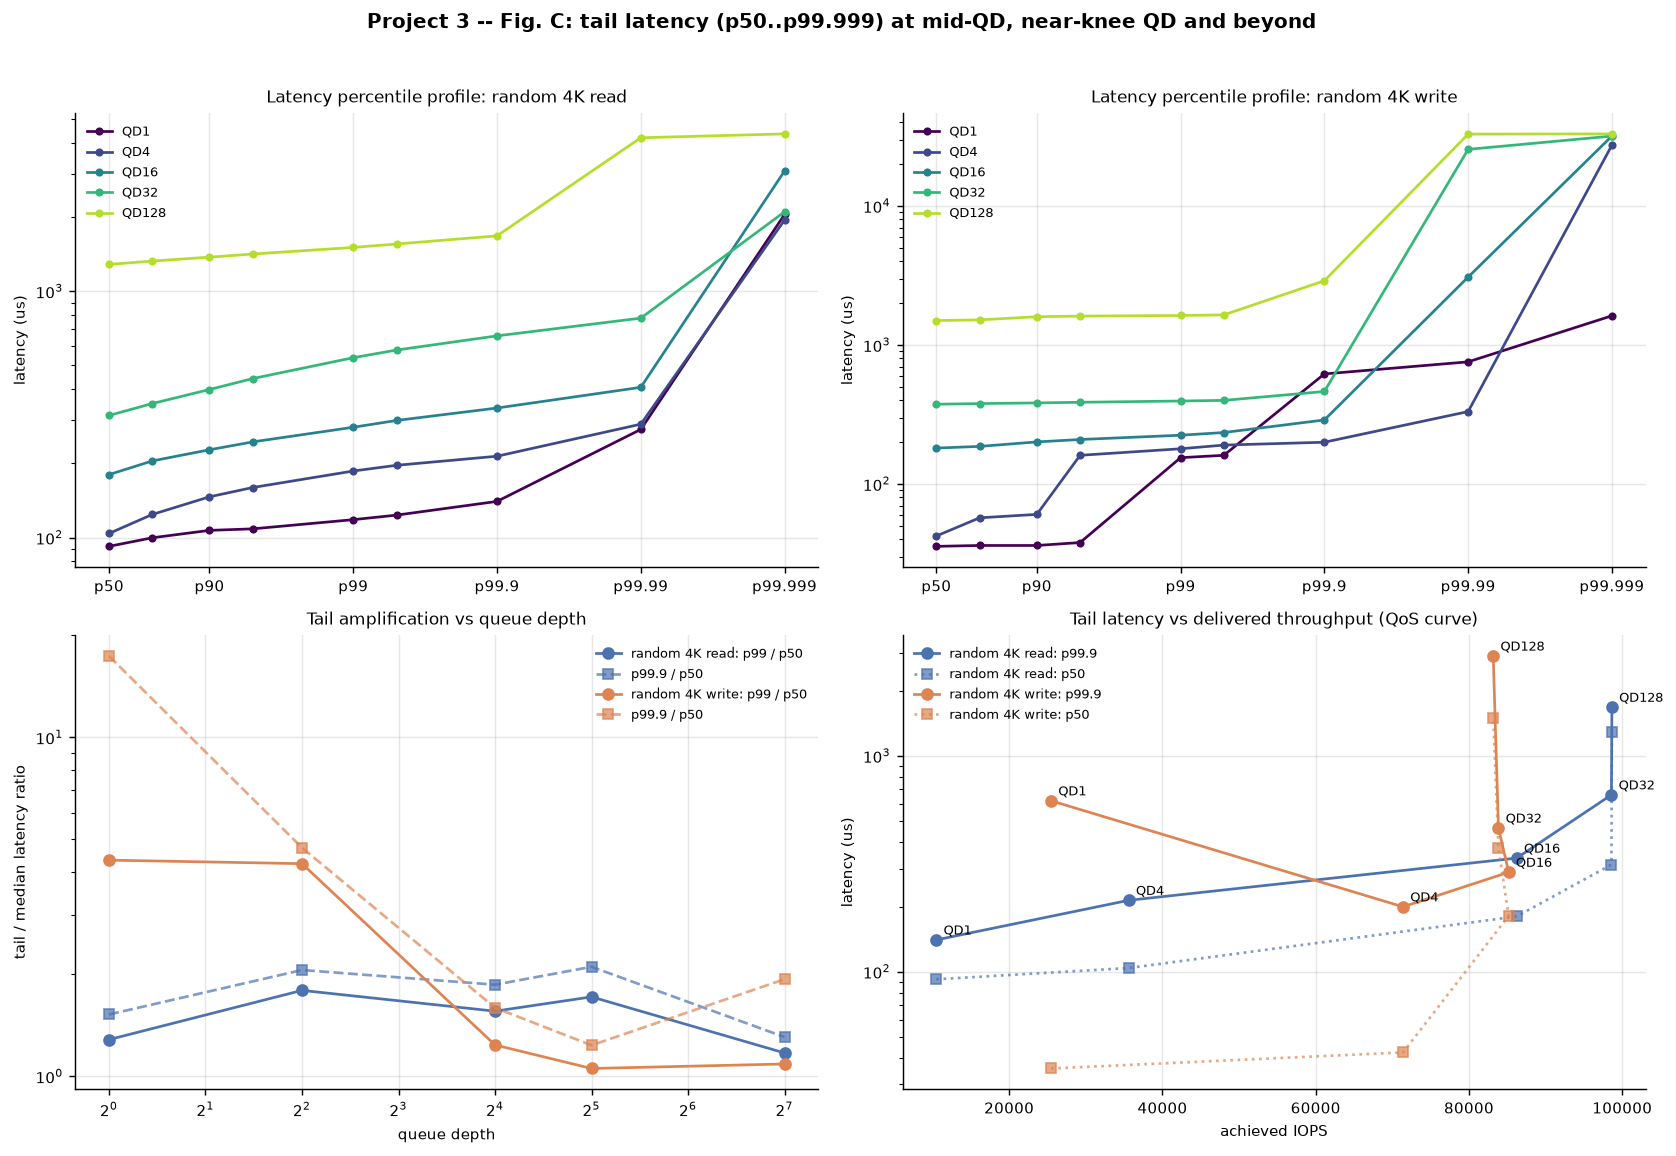
\includegraphics[width=\linewidth]{../results/figC_tail_latency.png}
\caption{Random 4\,KiB I/O, with percentile profiles from the median to the 99.999th percentile (top), tail amplification (bottom left) and the trade-off between tail latency and throughput (bottom right).}\label{fig:C}\end{figure}
Reads have a compact tail. At every QD the p99.9 stays within about twice the median, because reads have a deterministic service time and queueing only shifts the whole distribution (Tab.~\ref{tab:tail}, Fig.~\ref{fig:C}). Past the knee the profile is a shifted copy, and the rare outliers of a few ms do not depend on QD.

Writes differ. Their tail amplification is largest at low load, where a minority of writes hit an internal event. From QD16 up the median grows with queueing and the ratio shrinks, but the extreme tail does not, as the maximum latency is 30--48\,ms at every QD, a write-path stall the C++ tool also sees. It looks like controller housekeeping, such as flushing the write buffer or garbage collection; it is invisible to means and even to p99.9 at low QD, yet it dominates the tail of any write-heavy service. Queueing past the knee is pure loss. From QD32 to QD128 the read p99.9 grows 2.5$\times$ and the write p99.9 6.3$\times$ for no extra IOPS (Fig.~\ref{fig:C}, bottom right).

\subsection{Working set and data pattern}\label{sec:ws}
Random-read IOPS at QD32 fall a steady 1.9\% from a 1\,MiB LBA range to the whole 1500\,MiB file (Fig.~\ref{fig:D}b), and random writes do not depend on the range at all. The whole span is far smaller than what the drive's DRAM-cached mapping table covers, so capacity effects that a full-drive test could reveal are out of reach. A 90\%-compressible payload gives the same write throughput as incompressible data at QD32, 84.0 against 83.7\,k random 4\,KiB IOPS and 506 against 505\,MB/s sequential, so this drive does not compress; the payload was kept incompressible anyway, for comparability with drives that do.

\subsection{Burst vs.\ steady state, write cache and garbage collection}\label{sec:state}
\begin{figure}[!htb]\centering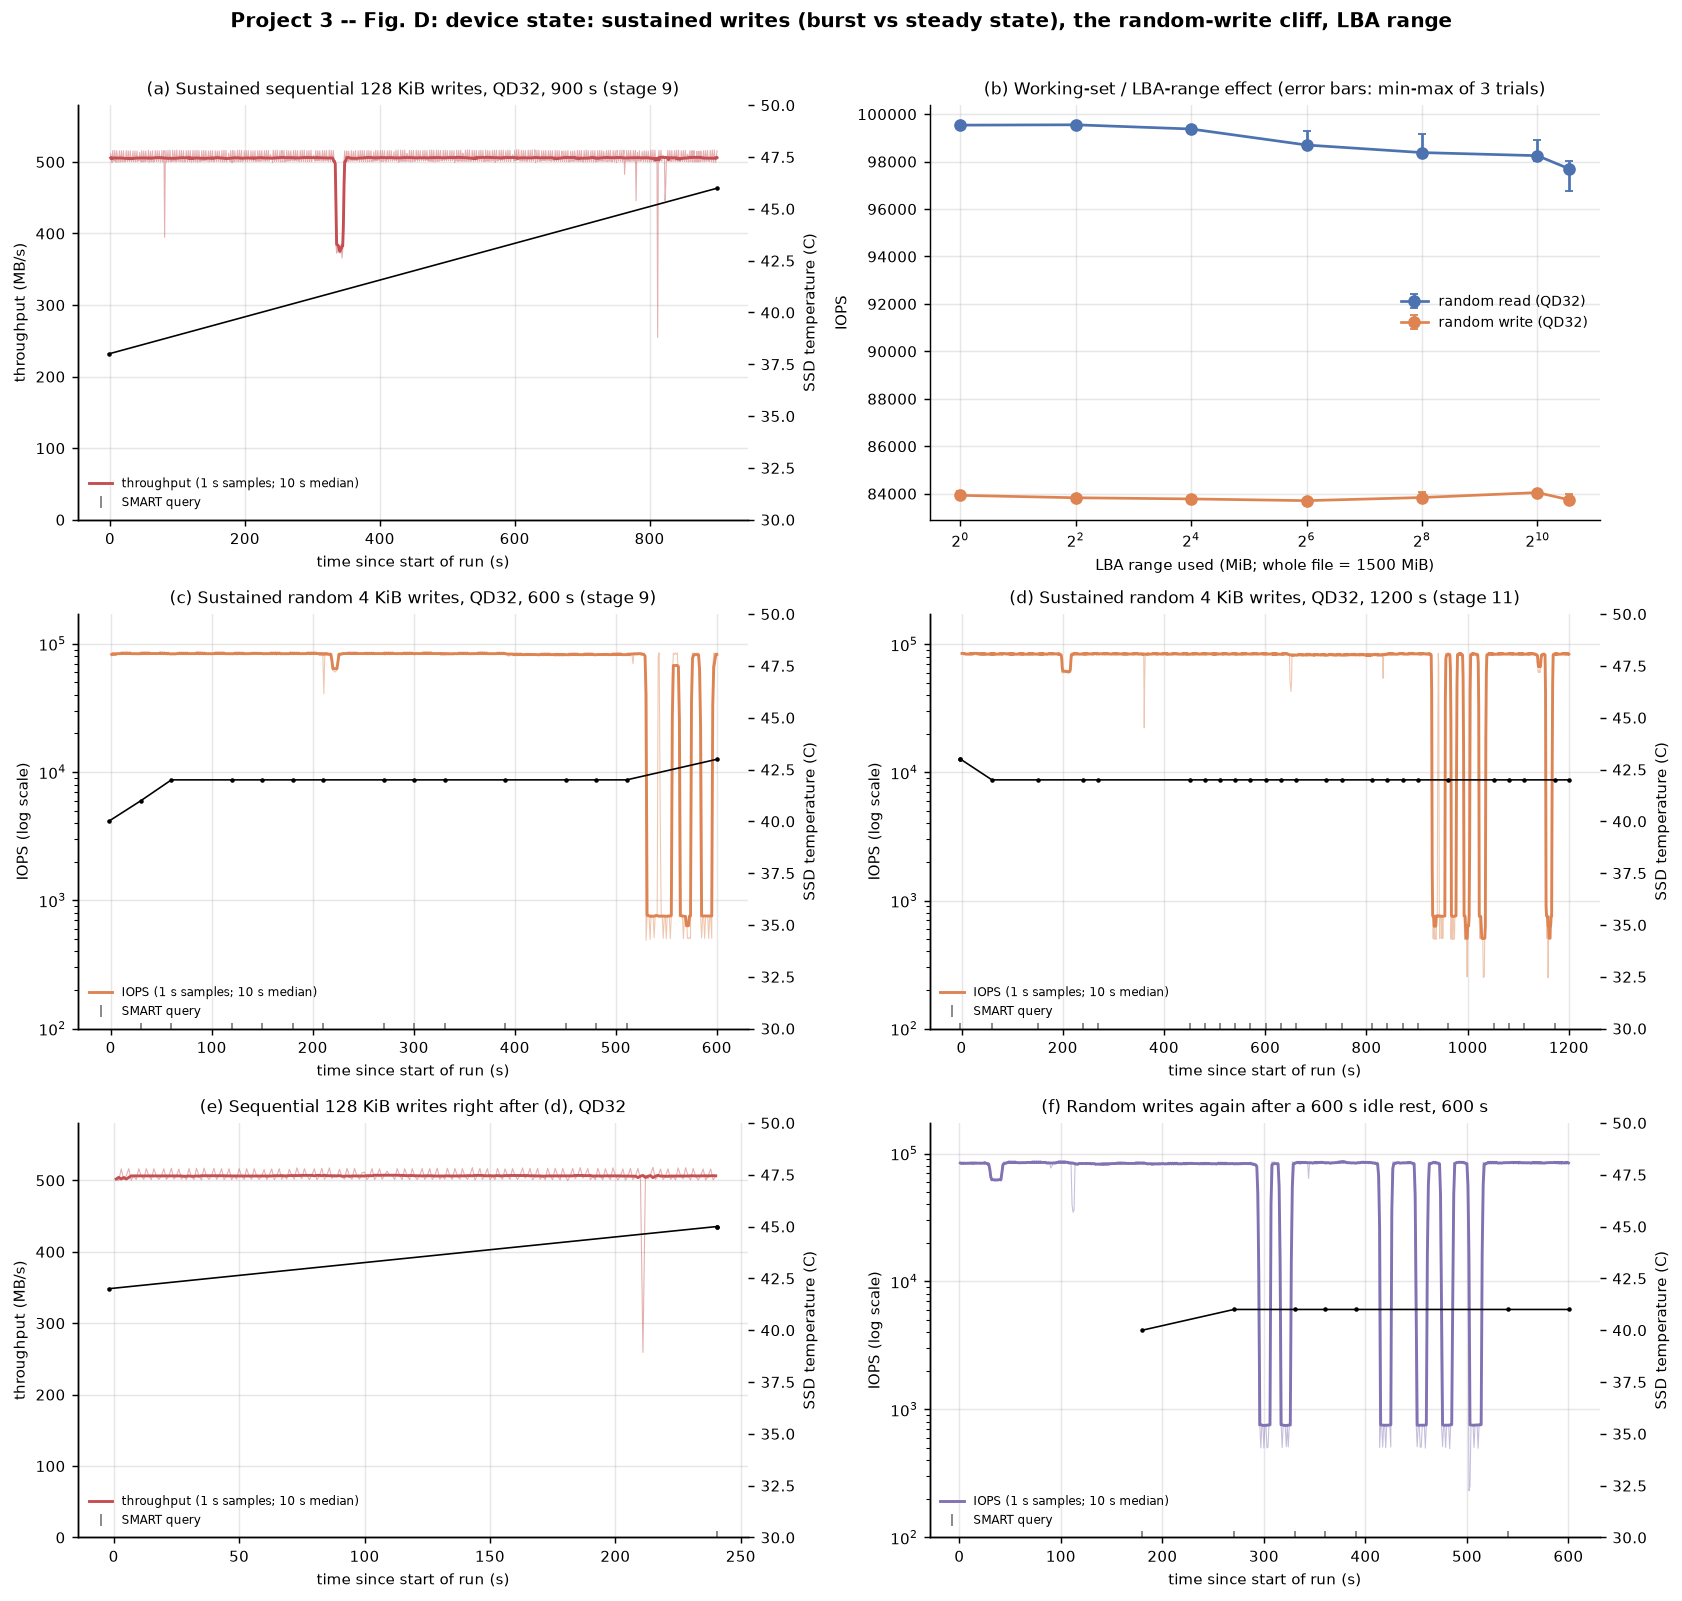
\includegraphics[width=0.9\linewidth]{../results/figD_device_state.png}
\caption{Device state, 1\,s samples thin and 10\,s medians thick; random-write IOPS on a log scale. (a) 900\,s of sequential 128\,KiB writes. (b) LBA-range effect, min--max of 3 trials. (c), (d), (f) sustained random 4\,KiB writes at queue depth 32 over the whole file, for 600\,s, 1200\,s, and 600\,s after a 600\,s idle rest. (e) Sequential writes right after (d). This figure alone wrote 1.3\,TB.}\label{fig:D}\end{figure}
\begin{table}[!htb]\centering\small\resizebox{\linewidth}{!}{%
\begin{tabular}{lrrrrr}
\toprule
sustained random 4\,KiB writes, QD32 & fast rate & first slow second & written before it & slow episodes & slow seconds after onset \\
\midrule
stage 9, 600\,s & 84.4\,k IOPS & 529\,s & 180\,GB & 4 $\times$ $\approx$12\,s & 68\% \\
stage 11 a, 1200\,s & 84.8\,k IOPS & 927\,s & 316\,GB & 6 $\times$ $\approx$12\,s & 28\% \\
stage 11 c, 600\,s after 10\,min idle & 83.7\,k IOPS & 293\,s & 99\,GB & 6 $\times$ $\approx$12\,s & 23\% \\
\bottomrule
\end{tabular}}
\caption{The write cliff. A slow second is one below 10\% of the fast rate; in every episode the drive completes about 750 IOPS, about 45\,ms of mean latency at queue depth 32.}\label{tab:cliff}\end{table}
Sequential writes show no burst-to-steady-state transition. A 900\,s run, 454\,GB or 300 times the file size, holds 505\,MB/s throughout apart from one 15\,s dip and two one-second dips (Fig.~\ref{fig:D}a), and sequential writes right after the random-write cliff are unaffected (Fig.~\ref{fig:D}e). This does not prove the SLC cache was never exhausted, because a review reports that the MX500 falls back from SLC to TLC mode after about 30\,GB of sequential writes \cite{computerbase}, so the flat rate, the SATA limit, is equally consistent with direct-to-TLC writing at or above the link rate.

Random writes, in contrast, show a cliff, but not an SLC-capacity one. At QD32 the drive sustains about 84\,k IOPS for 5--15 minutes, then alternates episodes of about 12\,s at only about 750 IOPS, a 110-fold collapse, with fast intervals of a few seconds (Fig.~\ref{fig:D}c, d, f; Tab.~\ref{tab:cliff}). The onset is not a fixed volume, and a 10-minute idle rest did not delay it. Since 99--316\,GB are 63--201 complete overwrites of the 1500\,MiB file, the valid data never exceeded 1500\,MiB, which excludes SLC exhaustion by unique data. The cliff is most likely steady-state garbage collection from overwriting a small span at a high rate; this is a hypothesis, because the host cannot observe garbage collection. Temperature does not explain it either, at 41--45\,$^{\circ}$C throughout. QD1 probes after the heavy writes and after a further 300\,s idle match the fresh ones, with medians unchanged at 36\us\ for writes and 92\us\ for reads and 99th percentiles within 13\% (\nolinkurl{data/processed/device_state_qd1.csv}). The cliff exists only under sustained high-rate writing, so a QD1 test would never reveal it. A 45\,s run reports a clean 84\,k IOPS with a sub-millisecond p99.9, while a 10--20-minute run of the same workload spends up to two thirds of its time after the onset at about 1\% of that rate. Whether a full drive shows the same cliff is open, because that test needs a partition the size of the SLC cache, which is not safe to create on a disk that also holds the data volume.

\subsection{Thermal behaviour and read-throughput stability}\label{sec:readstab}
\begin{figure}[!htb]\centering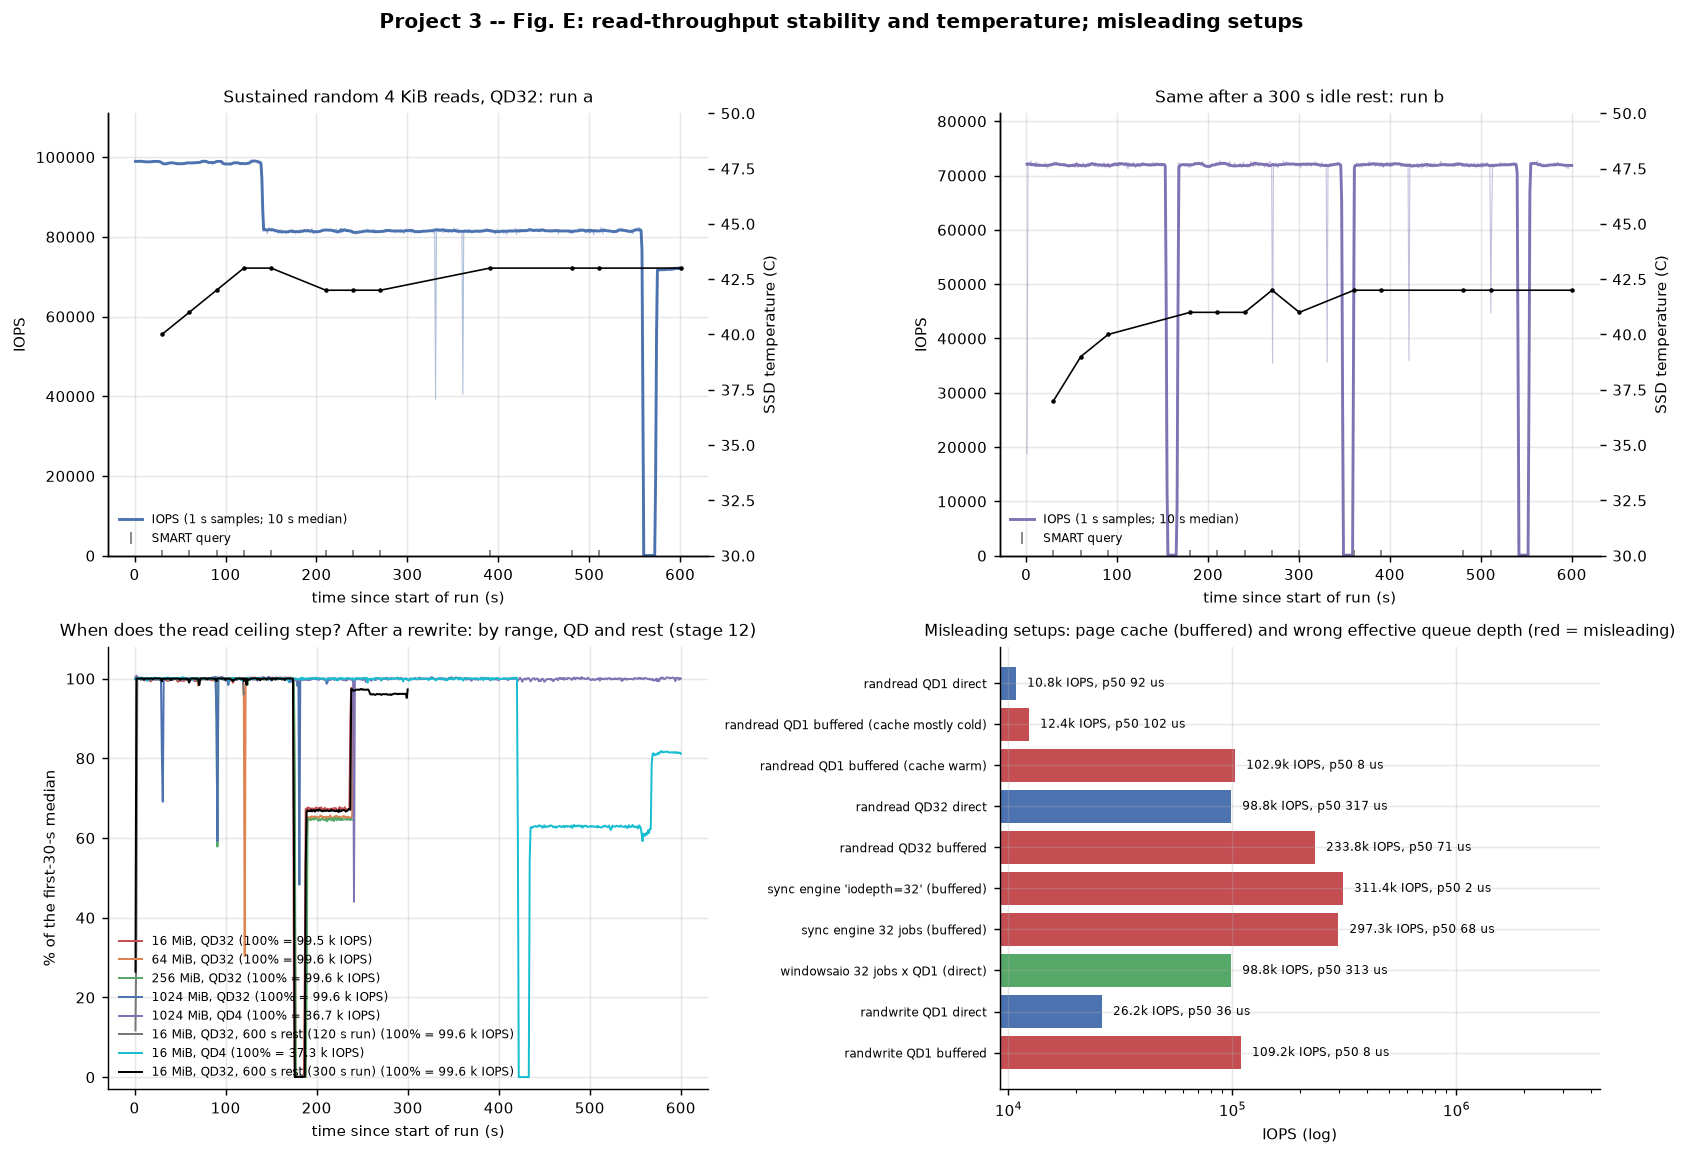
\includegraphics[width=\linewidth]{../results/figE_read_stability_and_pitfalls.png}
\caption{Sustained random 4\,KiB reads at queue depth 32 over 1\,GiB, runs a and b of stage 10, 1\,s samples thin and 10\,s medians thick, with the drive temperature in black where the query succeeded (top); reads after a full rewrite of the file, as a percentage of the first 30\,s, by range, queue depth and idle rest (bottom left); misleading setups of Sec.~\ref{sec:pitfalls} (bottom right).}\label{fig:E}\end{figure}
\begin{table}[!htb]\centering\small\resizebox{\linewidth}{!}{\begin{tabular}{lrrrrr}
\toprule
random 4 KiB reads after a full rewrite of the file & fast rate (k IOPS) & run length (s) & first stall (s) & reads before it (M) & rate after it (k IOPS) \\
\midrule
16 MiB, QD32 & 99.5 & 240 & 174 & 17.3 & 66.9 \\
64 MiB, QD32 & 99.6 & 240 & 175 & 17.4 & 65.0 \\
256 MiB, QD32 & 99.6 & 240 & 175 & 17.4 & 64.4 \\
1024 MiB, QD32 & 99.6 & 240 & none & (23.7 in total) & -- \\
1024 MiB, QD4 & 36.7 & 600 & none & (22.0 in total) & -- \\
16 MiB, QD32, 600 s rest (120 s run) & 99.6 & 120 & none & (11.8 in total) & -- \\
16 MiB, QD4 & 37.3 & 600 & 420 & 15.7 & 23.4 \\
16 MiB, QD32, 600 s rest (300 s run) & 99.6 & 300 & 174 & 17.2 & 66.6 \\
\bottomrule
\end{tabular}
}
\caption{When does the read ceiling step? Each run starts after a full sequential rewrite of the file and 60\,s of idle, or 600\,s in the rest runs. The first stall is the first second at which the 9\,s rolling median falls below 90\% of the first 30\,s; each is followed by about 12\,s at almost no throughput.}\label{tab:readstep}\end{table}
Long runs of random 4\,KiB reads test whether the read ceiling stays constant under sustained load and whether any change follows the drive's temperature (hypothesis 9).

In run a (Fig.~\ref{fig:E}, top left) the drive reads at full speed for about 140\,s, steps down by 17\%, stalls for about 13\,s several minutes later and settles lower still. Run b, started after a 300\,s idle rest, does not recover. It starts at the lower rate and stalls for about 12\,s every 193\,s. After a full rewrite of the file the reads are fast again and the same event follows. For ranges of 16, 64 and 256\,MiB at QD32 the first stall begins at the same second, lasts about 12\,s and leaves a plateau at about two thirds of the fast rate (Tab.~\ref{tab:readstep}).

Temperature does not explain the steps. The SSD warms smoothly and shows no change at any step or stall (Fig.~\ref{fig:E}), staying at 34--47\,$^{\circ}$C over the campaign, far below the listed 70\,$^{\circ}$C operating limit \cite{kabum}, which is an ambient limit rather than a documented throttling threshold. Hypothesis~9 is rejected for this sparse temperature reading; the drive's internal throttling state is not visible. Neither does the host, since the \texttt{PhysicalDisk} counters report reads per second equal to the measured rate and 30--32 requests outstanding, total processor load stays near 5\%, and no host counter, including interrupt and deferred procedure call time, shows the steps or stalls. Nor does the LBA range, since ranges 16 times apart stall at the same second.

The event scales with the reading rate. At QD4, which reads at about a third of the QD32 rate, the 16\,MiB run stalls 2.4 times later but after only 10\% fewer reads (Tab.~\ref{tab:readstep}), so the event follows a number of reads more closely than a time. There is one run per condition, and the five events of Tab.~\ref{tab:readstep} span 15.7--17.4 million reads. On 1\,GiB there was no stall within more than 22 million reads at either QD. A 600\,s idle rest after the rewrite neither made the drive start slow nor delayed the event, so idling does not reset the trigger and it does not depend on the time since the data were written.

Repeated reads disturb neighbouring flash cells, a documented effect that controllers must manage \cite{cai2015,cai2017}. The behaviour fits read-disturb management. After about 15--17 million reads of the same hot data the controller relocates it in one 12\,s burst that blocks the drive, and serves the relocated copy at about two thirds of the original rate, perhaps because it is stored differently; rewriting the file restores the fast layout. This is a hypothesis, not documented behaviour of this controller, and three observations do not fit it. The same read count on 1\,GiB produces no event, run b's periodic stalls come every 13.9 million reads, and run a stepped earlier, at about 13.6 million. The measurement consequence is established. A 4\,KiB random-read test of 8\,s, or even 2 minutes, reports the full rate, while the same drive delivers only 63--82\% of it, with 12\,s stalls, after a few minutes of continuous reading of a small hot set. The read tail of Tab.~\ref{tab:tail} is therefore a property of a state, not of the drive.

\section{Misleading setups and anomalies}\label{sec:pitan}
\subsection{Misleading setups (each measured)}\label{sec:pitfalls}
\begin{table}[!htb]\centering\small\begin{tabular}{lrrrrr}
\toprule
C++ reference (QD=1, synchronous) & ops/s & mean $\mu$s & p50 & p99 & p99.9 \\
\midrule
randread4k\_buffered & 13,803 & 72.4 & 92.2 & 121.2 & 168.7 \\
randread4k\_direct & 10,926 & 91.5 & 91.6 & 106.0 & 173.7 \\
randwrite4k\_buffered & 301,113 & 3.3 & 2.7 & 9.2 & 12.5 \\
randwrite4k\_direct & 28,194 & 35.4 & 33.2 & 152.5 & 165.8 \\
randwrite4k\_wt & 28,274 & 35.3 & 33.2 & 152.2 & 166.0 \\
seqread128k\_direct & 1,382 & 723.3 & 709.1 & 975.6 & 1163.4 \\
seqwrite128k\_direct & 3,412 & 293.1 & 273.8 & 396.3 & 426.2 \\
vdl\_unwritten\_file & 730,564 & 1.3 & 1.3 & 1.5 & 2.0 \\
vdl\_written\_file & 10,411 & 96.0 & 91.7 & 141.0 & 1339.5 \\
\bottomrule
\end{tabular}

\caption{Independent C++ tool, medians of 3 runs of 8--10\,s per mode over a 1\,GiB range, except the sparse-file test. The buffered and unwritten-file cases are the misleading ones; the buffered read is partly cold here.}\label{tab:ref}\end{table}
\begin{enumerate}
  \item The page cache inflates results, depending on how warm it is. With a 1\,GiB range, buffered 4\,KiB random reads at QD1 run near the direct-I/O rate while the cache is cold but almost ten times faster once the file is in memory, and buffered writes complete into the cache about four times faster than direct ones (Fig.~\ref{fig:E}, bottom right). A buffered test measures memory and the copy path, not the SSD, and its result depends on how much of the file happens to be cached. The C++ tool shows the same effect, and the write-through flag alone gives the same write rate as unbuffered writes (Tab.~\ref{tab:ref}).
  \item An unwritten, sparse file is never read from disk. Reading a freshly extended NTFS file never touches the disk, because unwritten ranges read as zeros \cite{mssparse}, and the C++ tool measures 70 times the rate of the same range once written. This is why the file is written twice before the first test.
  \item The effective queue depth can be wrong. FIO's synchronous engines ignore \texttt{iodepth} and on Windows cannot use direct I/O \cite{fiodoc}, so \texttt{ioengine=sync} with \texttt{iodepth=32} reports about three times the drive's real rate, all from the cache. The correct ways to get 32 outstanding requests, \texttt{windowsaio} with \texttt{iodepth=32} or 32 jobs at queue depth 1, give identical results, as Little's Law predicts.
  \item A single run, or a mean, misrepresents a state that moves. A sustained read run changes plateau after minutes (Sec.~\ref{sec:readstab}), so one 8\,s run or a mean of runs would be an arbitrary pick among the plateaus, and a 30\,s write test would never see the cliff of Sec.~\ref{sec:state}.
\end{enumerate}

\subsection{Honest anomalies}\label{sec:anomalies}
\begin{itemize}
  \item Large reads depend on how the range was last written. In every pure-read run of 16\,KiB or more, the reads are slow when the last writes to the range were 4\,KiB random writes and fast when they were 128\,KiB or larger. Stage 1 and the queue-depth sweep read a range last written by 4\,KiB random writes, where a 128\,KiB sequential read takes 720--830\us\ at QD1 and the plateau is about 390\,MB/s, close to the 4\,KiB random-read ceiling. The block-size and mix stages read after large writes, where the same read takes about 500\us\ and reaches the link limit. The block-size stage's re-run trial, taken after stage 9's random writes and stage 10's sustained reads, is 1.4--1.6 times slower for random 16--256\,KiB reads, so the medians in Tab.~\ref{tab:bs} come from the other two trials. 4\,KiB reads keep their 92\us\ median throughout. An untested explanation is that 4\,KiB random overwrites scatter each 128\,KiB range over 32 flash pages, so one large read costs as much as many small ones. Even in the fast case a QD1 read reaches under half of the link rate, because a direct read pays the full flash access before the next request is issued.
  \item Read-throughput steps and stalls under sustained load are not explained by temperature or host load, and are the same for ranges of 16--256\,MiB but absent on a freshly rewritten 1\,GiB range. Read-disturb management is the best-supported but untested explanation (Sec.~\ref{sec:readstab}).
  \item A write cliff appears after 99--316\,GB of random writes, with latency at QD1 unchanged afterwards (Sec.~\ref{sec:state}).
  \item Stalls of 0.1--1\,s in sequential-write jobs at QD1--4 that followed write-heavy random stages cost up to 98\% of a job's throughput (\nolinkurl{data/processed/stall_census.csv}), while 900\,s of sustained sequential writes at QD32 barely dip. Garbage collection of the freshly fragmented mapping is possible but untested.
  \item 4\,KiB sequential reads are slower than random reads at QD32, although every larger size matches. Four consecutive 4\,KiB blocks share a flash page and probably a die, so a sequential stream may keep fewer dies busy; untested.
  \item Writes complete in 36\us\ at QD1, far below a flash program time, because the drive acknowledges them from its volatile cache. Write-through gives the same rate, so no durable-write latency was measured.
  \item Write stalls of about 30\,ms at every QD and a small 2--3\,s oscillation in the per-second write rate, possibly periodic write-buffer flushes.
  \item Random writes decline slightly beyond QD16, and the 70/30 mix beyond QD64; the cause is not visible from the host.
  \item Drive-temperature queries fail under load and perturb the drive when frequent, so the temperature is known only at job boundaries and sparsely inside long runs.
\end{itemize}

\section{Use of artificial intelligence (AI)}\label{sec:aiuse}
Since Professor Tong Zhang has been encouraging the use of AI for learning, with an emphasis on how to best leverage it, I made an effort to experiment with the boundaries of how I used AI in this assignment.

Throughout this process, I used AI to teach myself about deeper technical detail concerning report topics. I used a mix of Qwen 3.8 running locally via OpenCode to build the repository and code. I used Claude Opus 5.0, 5.1, and 5.5 (they came out over the course of this semester) for technical questions.

Once I had a pipeline for getting results, I was able to independently tweak benchmarks and draw conclusions about my hypotheses. I rejected some charts that didn't make sense to me, and got the AI to combine other charts so data could be better viewed side by side.

I experimented with AI use beyond writing the benchmark code to varying degrees of success. One thing that went well was using Qwen to make charts and tables, most scripts that do this were written by Qwen.

One AI experiment that went wrong was when it came time to compile the final report from my independent hypotheses and findings. I gave Claude the documents and charts, and it immediately made 100+ pages of report across 3 projects. After a signifigant number of AI and human independent revisions, I managed to get this down to a more digestible $\approx$~40 pages accross all 3 projects. \textbf{This includes the clickable guides in the appendix, which were generated by AI to make the report more legible from the perspective of the handout, for easy grading.}


\begin{thebibliography}{9}
\raggedright\small
\bibitem{course} ECSE 4320/6320 Advanced Computer Systems, \emph{Class-wide Projects} (course document, due October 16): requirements and grading rubrics.
\bibitem{little1961} J.~D.~C. Little, ``A proof for the queuing formula: $L=\lambda W$,'' \emph{Operations Research} 9(3), 383--387, 1961. doi:10.1287/opre.9.3.383.
\bibitem{ocinside} OCinside.de, ``Crucial MX500 1\,TB SSD Review,'' page 2, manufacturer specifications, \url{https://www.ocinside.de/review/crucial_mx500_1tb_ssd/2/}.
\bibitem{geektopia} Geektopia, \emph{Crucial MX500 1\,TB} specification page, \url{https://www.geektopia.es/es/product/crucial/mx500-1-tb/} (a retailer-style listing, not the manufacturer).
\bibitem{kabum} KaBuM!, \emph{SSD Crucial MX500 1\,TB} (CT1000MX500SSD1) listing, \url{https://www.kabum.com.br/produto/94892/ssd-crucial-mx500-1tb-sata-leitura-560mb-s-gravacao-510mb-s-ct1000mx500ssd1}: operating temperature 0--70\,$^{\circ}$C.
\bibitem{computerbase} ComputerBase, ``Crucial MX500 im Test'' (2017), \url{https://www.computerbase.de/2017-12/crucial-mx500-ssd-test/}: 64-layer 3D TLC, dynamic SLC cache, TLC mode ``from a transfer size of about 30\,GB''.
\bibitem{ncq} ``Native Command Queuing,'' Wikipedia, \url{https://en.wikipedia.org/wiki/Native_Command_Queuing} (secondary source).
\bibitem{msfilebuf} Microsoft, ``File Buffering'' (Win32 documentation), \url{https://learn.microsoft.com/en-us/windows/win32/fileio/file-buffering}.
\bibitem{mssparse} Microsoft, ``Sparse Files'' (Win32 documentation), \url{https://learn.microsoft.com/en-us/windows/win32/fileio/sparse-files}.
\bibitem{msstorrel} Microsoft, \texttt{Get-StorageReliabilityCounter} (Storage module), \url{https://learn.microsoft.com/en-us/powershell/module/storage/get-storagereliabilitycounter}.
\bibitem{fiodoc} fio documentation, \url{https://fio.readthedocs.io/en/latest/fio_doc.html} (describes fio 3.42; this report used 3.43).
\bibitem{cai2015} Y.~Cai, Y.~Luo, S.~Ghose, E.~F. Haratsch, K.~Mai, O.~Mutlu, ``Read disturb errors in MLC NAND flash memory: characterization, mitigation, and recovery,'' \emph{IEEE/IFIP DSN}, 438--449, 2015, \url{https://ghose.cs.illinois.edu/papers/15dsn_readdisturb.pdf}.
\bibitem{cai2017} Y.~Cai, S.~Ghose, E.~F. Haratsch, Y.~Luo, O.~Mutlu, ``Error characterization, mitigation, and recovery in flash-memory-based solid-state drives,'' \emph{Proceedings of the IEEE} 105(9), 1666--1704, 2017, \url{https://arxiv.org/abs/1706.08642}.
\end{thebibliography}

\appendix
\section{Summary of results}\label{sec:summary}
{\small
\begin{tabular}{p{3.3cm}p{12.7cm}}
\toprule
\textbf{Question} & \textbf{Answer (evidence)} \\
\midrule
Latency at low load & At QD1, 4\,KiB random reads take about 90\us\ and writes under 40\us; a 128\,KiB sequential write takes little more than its transfer time, a read two to three times as long, depending on how the range was last written (Sec.~\ref{sec:anomalies}). The independent C++ tool agrees on every median (Tab.~\ref{tab:zq}, Fig.~\ref{fig:A}). \\
Peak throughput & Close to the manufacturer's figures in IOPS and in MB/s; large sequential transfers reach the SATA link limit (Tab.~\ref{tab:bs}). \\
Block size and pattern & IOPS fall and MB/s rise with block size until the link saturates at 64--128\,KiB. Random and sequential access match, except for small reads (Sec.~\ref{sec:bs}). \\
Read/write mix & At QD32, mixes with writes deliver under half of either pure workload (Tab.~\ref{tab:mix}). \\
Queue depth, knee and Little's Law & Reads saturate at QD32, the NCQ depth, and writes at QD8; beyond that only latency grows. The overlap $N^{*}$ from Little's Law is a lower bound for the knee (Tab.~\ref{tab:knee}, Fig.~\ref{fig:B}). \\
Tail latency & Read tails stay within about twice the median; writes stall for 30--48\,ms at every QD (Tab.~\ref{tab:tail}, Fig.~\ref{fig:C}). \\
Device state & Sequential writes hold their rate for 900\,s; sustained random writes fall off a cliff after 99--316\,GB; QD1 latency is unchanged afterwards; the LBA range matters little (Fig.~\ref{fig:D}, Tab.~\ref{tab:cliff}). \\
Thermal behaviour & The drive stayed at 34--47\,$^{\circ}$C. Read-throughput steps and stalls under sustained load do not follow temperature or host load and look like a read-count trigger, which is not established (Sec.~\ref{sec:readstab}, Fig.~\ref{fig:E}). \\
Misleading setups & Buffered I/O, a sparse file and a synchronous engine report 3--70 times the real rate (Sec.~\ref{sec:pitfalls}). \\
\bottomrule
\end{tabular}
}

\section{Where the rubric categories are answered}\label{sec:rubric}
\begin{center}\small
\begin{tabular}{p{6.0cm}rp{7.6cm}}
\toprule
\textbf{Rubric category} & \textbf{Points} & \textbf{Location} \\
\midrule
Safety and zero-queue baselines & 30 & Sec.~\ref{sec:safety} (safety), \ref{sec:zqsec} (baselines) \\
Block-size and pattern sweeps & 35 & Sec.~\ref{sec:bs} \\
Read/write and queue-depth analysis & 40 & Sec.~\ref{sec:mix}, \ref{sec:knee} \\
Tail latency and device state & 25 & Sec.~\ref{sec:tail}, \ref{sec:ws}, \ref{sec:state}, \ref{sec:readstab} \\
Reproducibility and data hygiene & 25 & Sec.~\ref{sec:repro}, \ref{sec:env}, \ref{sec:valid} \\
AI use transparency and pitfall analysis & 15 & Sec.~\ref{sec:aiuse} (AI use), \ref{sec:pitfalls} (pitfalls) \\
Report quality & 15 & whole report; checklist in App.~\ref{sec:checklist} \\
\bottomrule
\end{tabular}
\end{center}

\section{Requirements checklist}\label{sec:checklist}
Every requirement of the course document \cite{course} for Project~3 and its common requirements, with the section that answers it. \textbf{Met} = done and documented; \textbf{Partly} / \textbf{Not met} = not (fully) done and the reason is stated.
\begin{center}\footnotesize
\begin{longtable}{p{6.1cm}p{1.5cm}p{8.0cm}}
\toprule
\textbf{Requirement} & \textbf{Status} & \textbf{Where / evidence} \\
\midrule
\endhead
\multicolumn{3}{l}{\textit{Common requirements}} \\
AI-use note (tools, what was generated, what was modified/tested/rejected) & Met & Sec.~\ref{sec:aiuse} \\
Reproducible repository: FIO configs, scripts, raw results, parsed data, plotting code, README & Met & \texttt{data/raw/jobs|json|logs|ref}, \texttt{data/processed}, \texttt{scripts/}, \texttt{README.md}; Sec.~\ref{sec:repro} \\
Pre-experiment hypothesis & Met & Sec.~\ref{sec:hyp} (9 hypotheses, outcome stated) \\
Correctness validation & Met & Sec.~\ref{sec:valid} (independent C++ tool, identities on every run, parser self-test) \\
Measurement discipline: hardware, OS, tool versions, frequency, SMT, pinning, repetitions, error bars & Met & Sec.~\ref{sec:env}; error bars = min--max of trials in all figures. FIO threads are deliberately \emph{not} pinned (host effects checked with OS counters, Sec.~\ref{sec:readstab}) \\
Negative/failure case (misleading setup) & Met & Sec.~\ref{sec:pitfalls} (page cache, sparse file, effective queue depth, averaged plateaus) \\
Honest anomalies & Met & Sec.~\ref{sec:anomalies} \\
Optional graphics processing unit (GPU)/CUDA extension & Not attempted & optional \\
\midrule
\multicolumn{3}{l}{\textit{Safety}} \\
Never benchmark a partition with valuable data; use a dedicated partition / disposable file with direct I/O & Met & dedicated 1.6\,GiB partition \texttt{T:}, one scratch file, direct I/O, hard-coded refusal checks (Sec.~\ref{sec:safety}); \texttt{G:} never opened \\
\midrule
\multicolumn{3}{l}{\textit{Experiments and plots}} \\
Zero-queue baselines: QD=1 latency, 4\,KiB random R/W and 128\,KiB sequential R/W, p95/p99 & Met & Tab.~\ref{tab:zq}, Fig.~\ref{fig:A} \\
Max small-block IOPS and large-block sequential throughput & Met & Tab.~\ref{tab:bs}, Tab.~\ref{tab:knee} \\
Block-size sweep: 4, 16, 32, 64, 128, 256\,KiB (+512\,KiB, 1\,MiB sequential), random and sequential, throughput and latency from the same runs & Met & Tab.~\ref{tab:bs}, Fig.~\ref{fig:A} \\
Read/write mix sweep (100/0, 0/100, 70/30, 50/50) at fixed block size and pattern & Met & Tab.~\ref{tab:mix} (4\,KiB random, QD1 and QD32; 128\,KiB sequential in \texttt{rw\_mix} data) \\
Queue-depth/parallelism sweep 1--256: throughput-vs-latency curve, knee, Little's Law & Met & Fig.~\ref{fig:B}, Tab.~\ref{tab:knee} (iodepth and numjobs) \\
Tail latency p95/p99/p99.9 at mid-QD and near-knee QD & Met & Tab.~\ref{tab:tail}, Fig.~\ref{fig:C} (QD 1, 4, 16, 32, 128; p50 to p99.999) \\
Working-set/LBA-range note & Met & Sec.~\ref{sec:ws}, Fig.~\ref{fig:D}(b) (1\,MiB to 1500\,MiB) \\
Device state: burst vs.\ steady state, temperature, SLC cache, garbage collection & Met & Sec.~\ref{sec:state} (900\,s sequential and 600/1200\,s random writes, $>$1\,TB written; SMART temperature at every job), Sec.~\ref{sec:readstab} \\
Data pattern: incompressible vs.\ compressible, consistent and documented & Met & Sec.~\ref{sec:ws} \\
One misleading setup demonstrated or explained & Met & Sec.~\ref{sec:pitfalls} (four, measured) \\
\midrule
\multicolumn{3}{l}{\textit{Deliverables}} \\
Methodology: SSD model, interface, filesystem vs.\ raw device, direct I/O, capacity/range used, OS, CPU, temperature & Met & Sec.~\ref{sec:method} (safe setup, environment table) \\
Plots/tables with units, error bars, fixed vs.\ varied knobs labelled & Met & all figures \\
Analysis grounded in queueing theory, controller behaviour, interface ceilings, tail-latency implications & Met & Sec.~\ref{sec:knee} (Little's Law, $N^{*}$), Sec.~\ref{sec:state}, Sec.~\ref{sec:tail} \\
\bottomrule
\end{longtable}
\end{center}

\end{document}
